\documentclass[tikz,border=4pt]{standalone}
\usepackage{amsmath}
\usepackage{xcolor}
\usetikzlibrary{arrows.meta,positioning,fit,calc,backgrounds}

\definecolor{ink}{HTML}{19232C}
\definecolor{subink}{HTML}{5B6872}
\definecolor{canvas}{HTML}{F8FAFC}
\definecolor{orange}{HTML}{D97706}
\definecolor{orangebg}{HTML}{FFF8F0}
\definecolor{green}{HTML}{168A50}
\definecolor{greenbg}{HTML}{F2FBF5}
\definecolor{blue}{HTML}{2767D4}
\definecolor{bluebg}{HTML}{F2F6FD}
\definecolor{red}{HTML}{D83C48}
\definecolor{grayedge}{HTML}{77838D}

\begin{document}
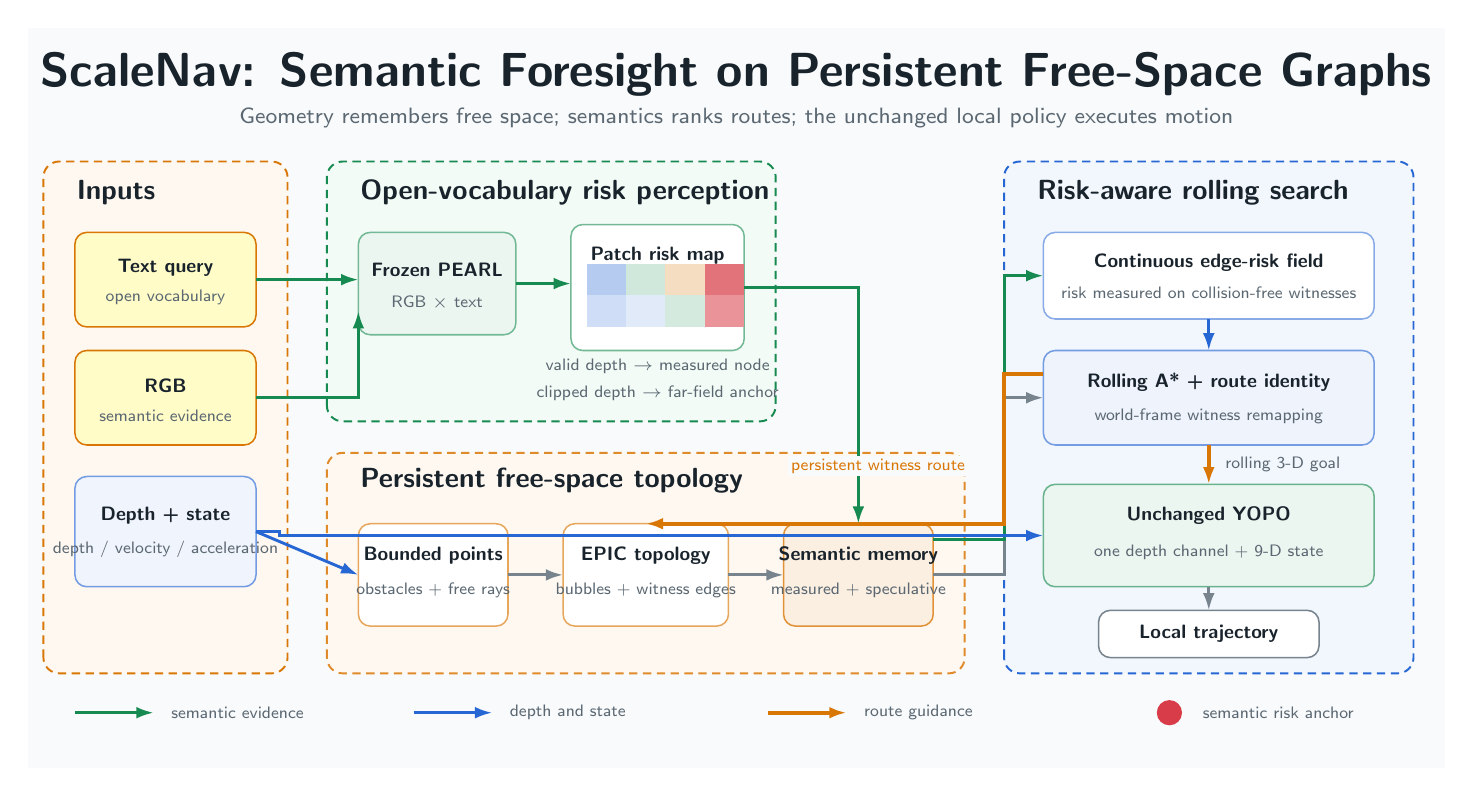
\begin{tikzpicture}[
  x=1mm,y=1mm,
  font=\sffamily,
  title/.style={font=\sffamily\bfseries\fontsize{17}{19}\selectfont,text=ink},
  subtitle/.style={font=\sffamily\fontsize{8}{10}\selectfont,text=subink},
  group/.style={font=\sffamily\bfseries\fontsize{10}{12}\selectfont,text=ink},
  nodetitle/.style={font=\sffamily\bfseries\fontsize{7.3}{8.6}\selectfont,text=ink,align=center},
  note/.style={font=\sffamily\fontsize{5.7}{7}\selectfont,text=subink,align=center},
  panel/.style={rounded corners=2mm,line width=.7pt,dashed,dash pattern=on 3pt off 2pt},
  box/.style={rounded corners=1.5mm,line width=.55pt,align=center,minimum height=13mm},
  flow/.style={-{Latex[length=2.2mm,width=1.5mm]},line width=1.05pt,draw=grayedge},
  semantic/.style={flow,draw=green},
  depth/.style={flow,draw=blue},
  route/.style={flow,draw=orange,line width=1.35pt}
]
\fill[canvas] (-2,-5) rectangle (178,89);
\node[title] at (88,83) {ScaleNav: Semantic Foresight on Persistent Free-Space Graphs};
\node[subtitle] at (88,77.5) {Geometry remembers free space; semantics ranks routes; the unchanged local policy executes motion};

% Inputs
\filldraw[panel,fill=orangebg,draw=orange] (0,7) rectangle (31,72);
\node[group,anchor=west] at (3,68) {Inputs};
\filldraw[box,fill=yellow!22,draw=orange] (4,51) rectangle (27,63);
\node[nodetitle] at (15.5,58.5) {Text query};
\node[note] at (15.5,54.7) {open vocabulary};
\filldraw[box,fill=yellow!22,draw=orange] (4,36) rectangle (27,48);
\node[nodetitle] at (15.5,43.5) {RGB};
\node[note] at (15.5,39.7) {semantic evidence};
\filldraw[box,fill=blue!7,draw=blue!65] (4,18) rectangle (27,32);
\node[nodetitle] at (15.5,27) {Depth + state};
\node[note] at (15.5,22.7) {depth / velocity / acceleration};

% Semantic perception
\filldraw[panel,fill=greenbg,draw=green] (36,39) rectangle (93,72);
\node[group,anchor=west] at (39,68) {Open-vocabulary risk perception};
\filldraw[box,fill=green!8,draw=green!60] (40,50) rectangle (60,63);
\node[nodetitle] at (50,58.3) {Frozen PEARL};
\node[note] at (50,54.1) {RGB $\times$ text};
\filldraw[box,fill=white,draw=green!60] (67,48) rectangle (89,64);
\node[nodetitle] at (78,60) {Patch risk map};
\foreach \x/\y/\c in {69/51/blue!22,74/51/blue!14,79/51/green!18,84/51/red!55,
                        69/55/blue!34,74/55/green!20,79/55/orange!25,84/55/red!72} {
  \fill[\c] (\x,\y) rectangle ++(5,4);
}
\node[note] at (78,46) {valid depth $\rightarrow$ measured node};
\node[note] at (78,42.6) {clipped depth $\rightarrow$ far-field anchor};
\draw[semantic] (60,56.5) -- (67,56.5);

% Persistent graph
\filldraw[panel,fill=orangebg,draw=orange!85] (36,7) rectangle (117,35);
\node[group,anchor=west] at (39,31.5) {Persistent free-space topology};
\filldraw[box,fill=white,draw=orange!65] (40,13) rectangle (59,26);
\node[nodetitle] at (49.5,22) {Bounded points};
\node[note] at (49.5,17.5) {obstacles + free rays};
\filldraw[box,fill=white,draw=orange!65] (66,13) rectangle (87,26);
\node[nodetitle] at (76.5,22) {EPIC topology};
\node[note] at (76.5,17.5) {bubbles + witness edges};
\filldraw[box,fill=orange!12,draw=orange!80] (94,13) rectangle (113,26);
\node[nodetitle] at (103.5,22) {Semantic memory};
\node[note] at (103.5,17.5) {measured + speculative};
\draw[flow] (59,19.5) -- (66,19.5);
\draw[flow] (87,19.5) -- (94,19.5);

% Search
\filldraw[panel,fill=bluebg,draw=blue] (122,7) rectangle (174,72);
\node[group,anchor=west] at (125,68) {Risk-aware rolling search};
\filldraw[box,fill=white,draw=blue!55] (127,52) rectangle (169,63);
\node[nodetitle] at (148,59.2) {Continuous edge-risk field};
\node[note] at (148,55.3) {risk measured on collision-free witnesses};

\filldraw[box,fill=blue!8,draw=blue!65] (127,36) rectangle (169,48);
\node[nodetitle] at (148,44) {Rolling A* + route identity};
\node[note] at (148,39.6) {world-frame witness remapping};
\draw[depth] (148,52) -- (148,48);

\filldraw[box,fill=green!8,draw=green!65] (127,18) rectangle (169,31);
\node[nodetitle] at (148,27) {Unchanged YOPO};
\node[note] at (148,22.4) {one depth channel + 9-D state};
\draw[route] (148,36) -- node[note,right,xshift=.7mm] {rolling 3-D goal} (148,31);

\filldraw[box,fill=white,draw=grayedge] (134,9) rectangle (162,15);
\node[nodetitle] at (148,12) {Local trajectory};
\draw[flow] (148,18) -- (148,15);

% Cross-panel flows
\draw[semantic] (27,57) -- (40,57);
\draw[semantic] (27,42) -| (40,53);
\draw[depth] (27,25) -- (40,19.5);
\draw[semantic] (89,56) -| (103.5,26);
\draw[flow] (113,19.5) -- (122,19.5) |- (127,42);
\draw[semantic] (113,24) -- (122,24) |- (127,57.5);
\draw[depth] (27,25) -- ++(3,0) |- (127,24.5);

% World-memory return
\draw[route] (127,45) -- ++(-5,0) |- (76.5,26);
\node[note,text=orange,fill=canvas,inner sep=1pt] at (106,33.3) {persistent witness route};

% Legend
\draw[semantic] (4,2) -- (14,2); \node[note,anchor=west] at (15,2) {semantic evidence};
\draw[depth] (47,2) -- (57,2); \node[note,anchor=west] at (58,2) {depth and state};
\draw[route] (92,2) -- (102,2); \node[note,anchor=west] at (103,2) {route guidance};
\fill[red] (143,2) circle (1.6mm); \node[note,anchor=west] at (146,2) {semantic risk anchor};
\end{tikzpicture}
\end{document}
